\documentclass[
  bibliography=totoc,     % Literatur im Inhaltsverzeichnis
  captions=tableheading,  % Tabellenüberschriften
  titlepage=firstiscover, % Titelseite ist Deckblatt
]{scrartcl}

% Paket float verbessern
\usepackage{scrhack}

% Warnung, falls nochmal kompiliert werden muss
\usepackage[aux]{rerunfilecheck}

% unverzichtbare Mathe-Befehle
\usepackage{amsmath}
% viele Mathe-Symbole
\usepackage{amssymb}
% Erweiterungen für amsmath
\usepackage{mathtools}

% Fonteinstellungen
\usepackage{fontspec}
% Latin Modern Fonts werden automatisch geladen
% Alternativ zum Beispiel:
%\setromanfont{Libertinus Serif}
%\setsansfont{Libertinus Sans}
%\setmonofont{Libertinus Mono}

% Wenn man andere Schriftarten gesetzt hat,
% sollte man das Seiten-Layout neu berechnen lassen
\recalctypearea{}

% deutsche Spracheinstellungen
\usepackage[ngerman]{babel}


\usepackage[
  math-style=ISO,    % ┐
  bold-style=ISO,    % │
  sans-style=italic, % │ ISO-Standard folgen
  nabla=upright,     % │
  partial=upright,   % │
  mathrm=sym,        % ┘
  warnings-off={           % ┐
    mathtools-colon,       % │ unnötige Warnungen ausschalten
    mathtools-overbracket, % │
  },                       % ┘
]{unicode-math}

% traditionelle Fonts für Mathematik
\setmathfont{Latin Modern Math}
% Alternativ zum Beispiel:
%\setmathfont{Libertinus Math}

\setmathfont{XITS Math}[range={scr, bfscr}]
\setmathfont{XITS Math}[range={cal, bfcal}, StylisticSet=1]

% Zahlen und Einheiten
\usepackage[
  locale=DE,                   % deutsche Einstellungen
  separate-uncertainty=true,   % immer Unsicherheit mit \pm
  per-mode=symbol-or-fraction, % / in inline math, fraction in display math
]{siunitx}

% chemische Formeln
\usepackage[
  version=4,
  math-greek=default, % ┐ mit unicode-math zusammenarbeiten
  text-greek=default, % ┘
]{mhchem}

% richtige Anführungszeichen
\usepackage[autostyle]{csquotes}

% schöne Brüche im Text
\usepackage{xfrac}

% Standardplatzierung für Floats einstellen
\usepackage{float}
\floatplacement{figure}{htbp}
\floatplacement{table}{htbp}

% Floats innerhalb einer Section halten
\usepackage[
  section, % Floats innerhalb der Section halten
  below,   % unterhalb der Section aber auf der selben Seite ist ok
]{placeins}

% Seite drehen für breite Tabellen: landscape Umgebung
\usepackage{pdflscape}

% Captions schöner machen.
\usepackage[
  labelfont=bf,        % Tabelle x: Abbildung y: ist jetzt fett
  font=small,          % Schrift etwas kleiner als Dokument
  width=0.9\textwidth, % maximale Breite einer Caption schmaler
]{caption}
% subfigure, subtable, subref
\usepackage{subcaption}

% Grafiken können eingebunden werden
\usepackage{graphicx}

% schöne Tabellen
\usepackage{tabularray}
\UseTblrLibrary{booktabs, siunitx}

% Verbesserungen am Schriftbild
\usepackage{microtype}

% Literaturverzeichnis
\usepackage[
  backend=biber,
]{biblatex}
% Quellendatenbank
\addbibresource{lit.bib}
\addbibresource{programme.bib}

% Hyperlinks im Dokument
\usepackage[
  german,
  unicode,        % Unicode in PDF-Attributen erlauben
  pdfusetitle,    % Titel, Autoren und Datum als PDF-Attribute
  pdfcreator={},  % ┐ PDF-Attribute säubern
  pdfproducer={}, % ┘
]{hyperref}
% erweiterte Bookmarks im PDF
\usepackage{bookmark}

% Trennung von Wörtern mit Strichen
\usepackage[shortcuts]{extdash}

\author{%
  Vincent Wirsdörfer\\%
  \href{mailto:vincent.wirsdoerfer@udo.edu}{authorA@udo.edu}%
  \and%
  Joris Daus\\%
  \href{mailto:joris.daus@udo.edu}{authorB@udo.edu}%
}
\publishers{TU Dortmund – Fakultät Physik}


\begin{document}
\section{Diskussion}
\label{sec:Diskussion}

Der Literaturwert \cite{Elementarladung} der Elementarladung $e0$ liegt näherungsweise bei 

\begin{equation*}
    e0 = 1.602\,176\,634\cdot{}10^{-19}\,\unit{\coulomb}.
\end{equation*}

\noindent Dementsprechend liegen die gemessenen Werte der Elementarladung sowohl mit als auch ohne Cunningham-Korrekturterm 

\begin{align*}
    q            &= \left(1.629\pm0.012\right)\cdot10^{-19}\,\unit{\coulomb} \\
    q_\text{eff} &= \left(1.590 \pm0.040\right)\cdot10^{-19}\,\unit{\coulomb} 
\end{align*}

in einer sehr kleinen Umgebung um den tatsächlichen Wert. Dieses Ergebnis weist prinzipiell auf eine gelungene und 
erfolgreiche Versuchsdurchführung hin. Nichtsdestotrotz ist beim Experimentieren ein breites Spektrum an systematischen 
Fehlern zum Vorschein getreten, welche im Folgenden näher diskutiert werden.\\

\noindent Die Zeitmessung der Öltröpfchen erfolgt über ein Mikroskop. Hierbei kann es zum Beschlagen des Objektivs 
kommen, was die Sicht auf die Tröpfchen partiell stark einschränken. Zusätzlich werden auf diese Art und Weise 
Parallaxenfehler begünstigt. Auch die Überanstrengung des Auges kann, speziell zum Ende des Versuchs, Einfluss auf die 
Messung haben und ggf. Ergebnisse verfälschen. Ferner betragen die Fall- und Steigzeiten der Öltröpfchen zumeist nur 
wenige Sekunden. Die Durchgabe der Zeiten und die daraus resultierende verzögerte Reaktionszeit hat also einen erheblichen 
Einfluss auf die Zeiten und somit auch auf die Geschwindigkeiten, welche essenziell für die Messung der Ladung sind.\\

\noindent Die Akkumulation der eben genannten Fehlerquellen sorgen für eine hohe Streuung der Werte und haben somit 
eine große Standardabweichung des Mittelwertes zur Folge. Diese lässt sich an den breiten Fehlerbalken in den Diagrammen 
im Kapitel \ref{sec:Auswertung} erkennen. Wie in \autoref{fig:Ladungsverteilung} zu sehen ist, erstreckt sich der Fehler 
einiger Ladungen um über das 16-fache der Elementarladung. Diese großen Unsicherheiten haben zur Folge, dass keine 
Häufungswerte ersichtlich werden. Bei einer theoretischen Zuordnung zu einem Häufungswert wären die Ladungen in mehreren 
Häufungswerten gleichzeitig. Dies ist keine sinnvolle Methode. Aufgrund der eben genannten Probleme können keine 
verlässlichen Werte durch gemeinsame Teiler bestimmt werden. Es muss daher auf den Literaturwert der Elementarladung 
zurückgegriffen werden, um weiter Ergebnisse zu bestimmen. Dieser wird jedoch nur als kleinster Teiler genommen. 


\section{Anhang}

Im Laborbuch wurden die folgenden Werte protokolliert.

\begin{figure}
    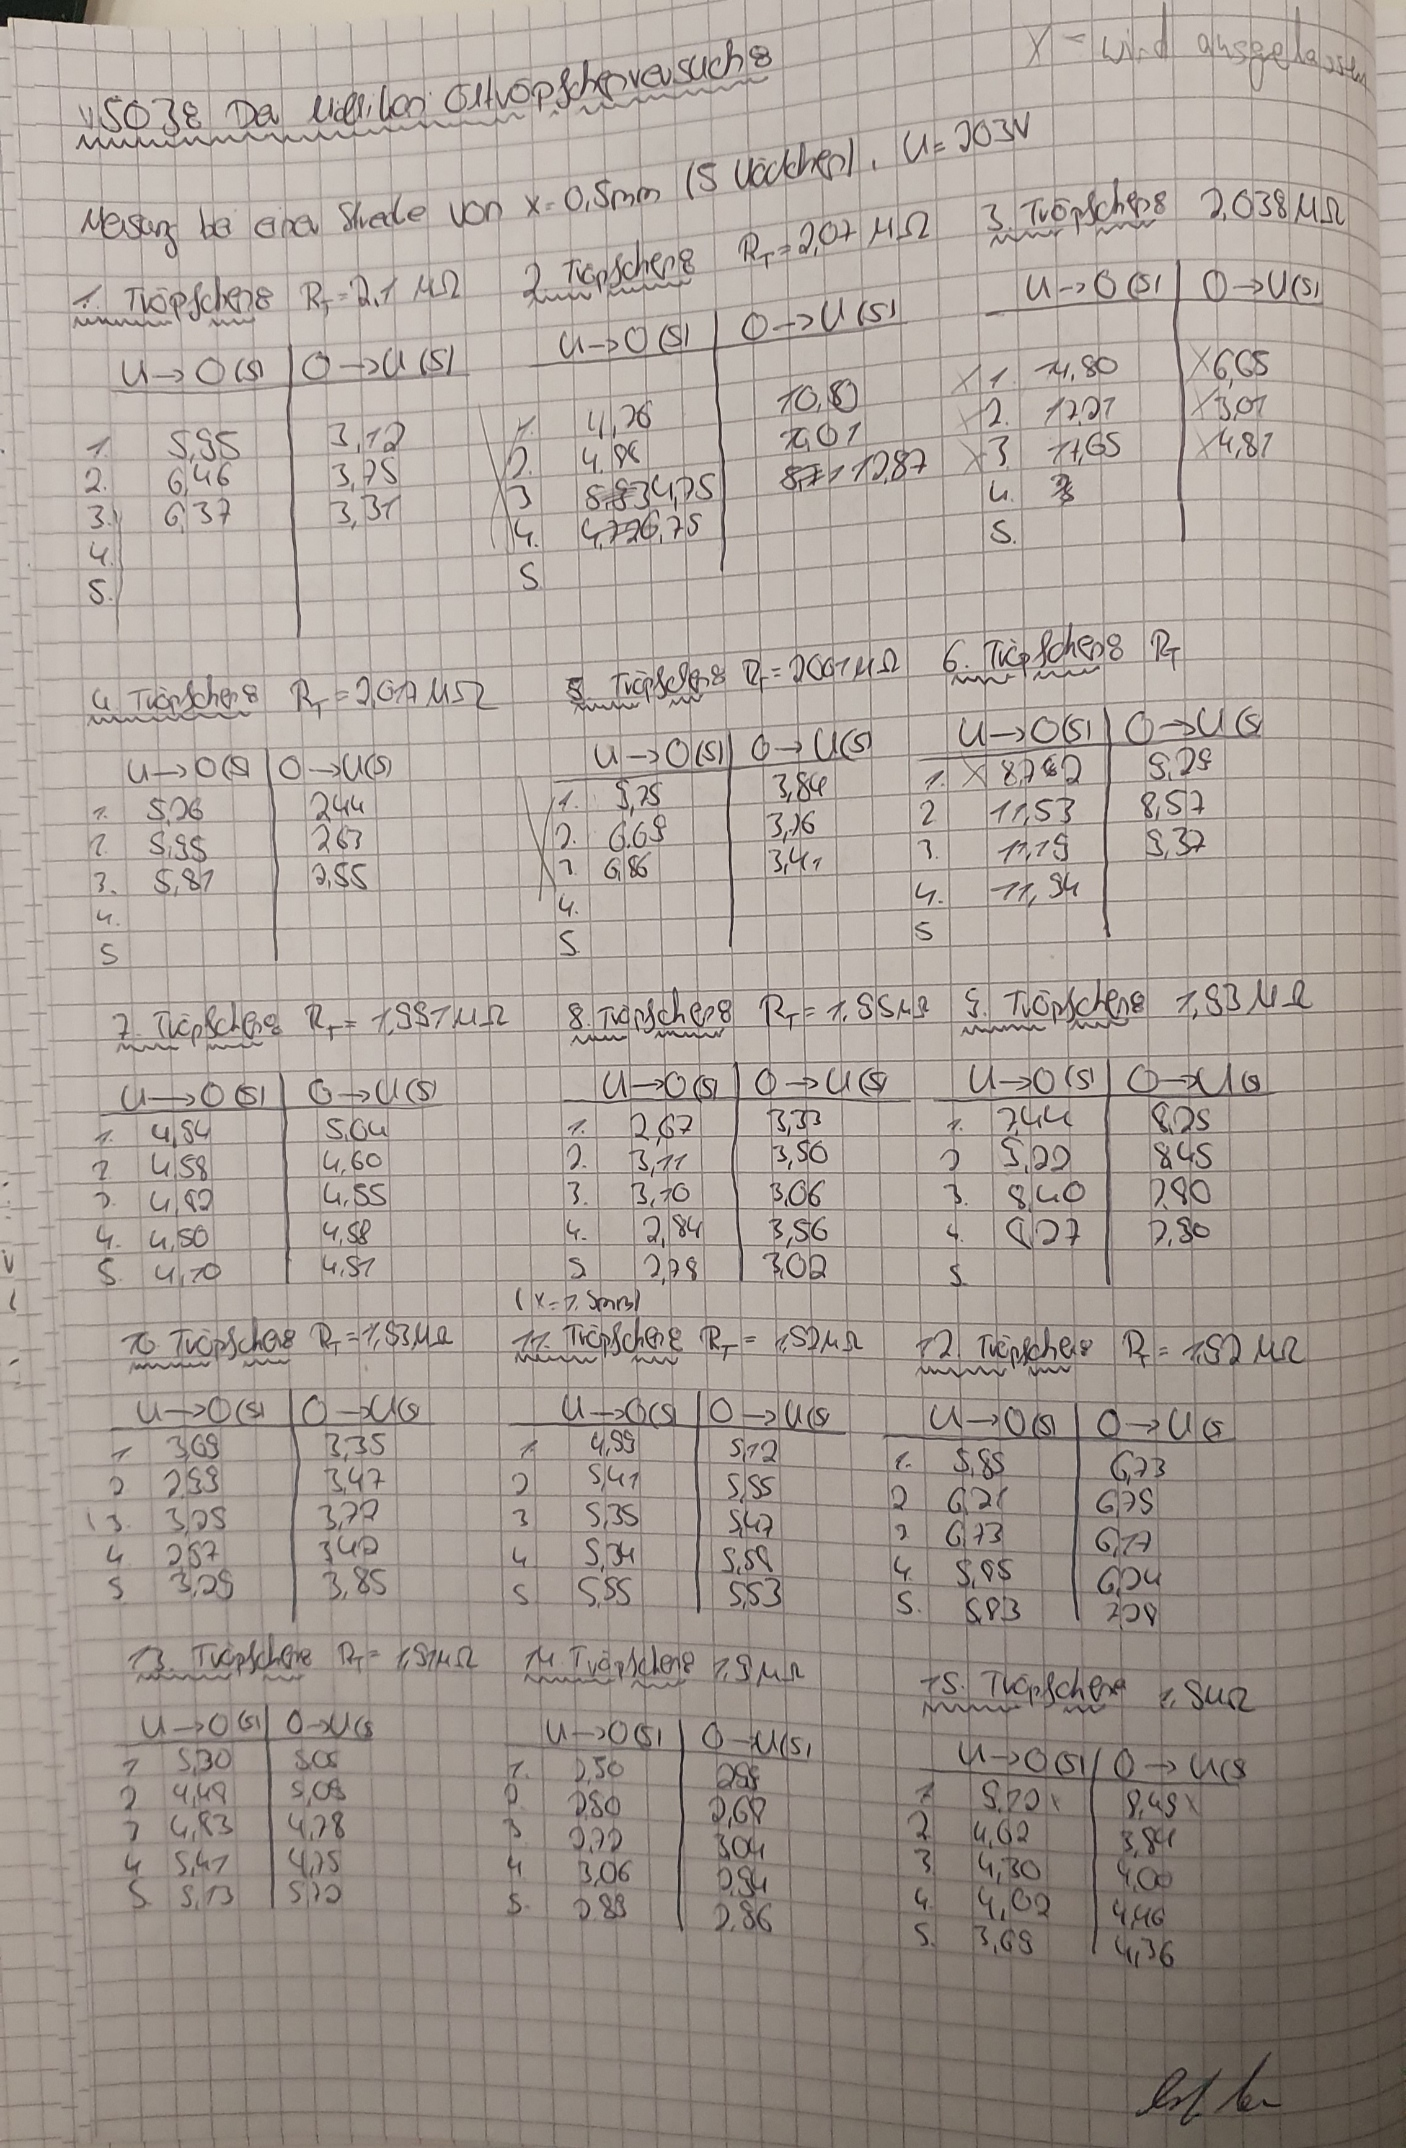
\includegraphics[width=14cm]{Laborbuch.jpg}
    \caption{Werte aus dem Laborbuch}
\end{figure}

\end{document}













%Ladung ändert sich durch Korrektur teilweise um ein e
%durch große Fehlerbalken keine Häufungswerte erkennbar
%Objektiv bei Versuchsdurchführung beschlagen
%Gegenlicht hat Tröpfchenbeobachtung erschwert
%systematischer Fehler durch Start-Stop ansagen
%für Auswertung quantisierung der Elementarladung und deren Wert benutzt, da sonst nicht anders möglich (weil zu große Fehler)
Wie in \autoref{fig:Ladungsverteilung} zu sehen ist, erstreckt sich der Fehler einiger Ladungen um über das 16-fache der Elementarladung. 
Diese großen Unsicherheiten haben zur Folge, dass keine Häufungswerte ersichtlich werden. Bei einer theoretischen Zuordnung zu einem Häufungswert wären 
die Ladungen in mehreren Häufungswerten gleichzeitig. Dies ist keine sinnvolle Methode.
Aufgrund der eben genannten Probleme können keine verlässlichen Werte durch gemeinsame Teiler bestimmt werden. Es muss daher auf den 
Literaturwert der Elementarladung zurückgegriffen werden, um weiter Ergebnisse zu bestimmen. Dieser wird jedoch nur als kleinster Teiler genommen. 

